\documentclass{beamer}

\pdfmapfile{+sansmathaccent.map}


\mode<presentation>
{
  \usetheme{Warsaw} % or try Darmstadt, Madrid, Warsaw, Rochester, CambridgeUS, ...
  \usecolortheme{seahorse} % or try seahorse, beaver, crane, wolverine, ...
  \usefonttheme{serif}  % or try serif, structurebold, ...
  \setbeamertemplate{navigation symbols}{}
  \setbeamertemplate{caption}[numbered]
} 


%%%%%%%%%%%%%%%%%%%%%%%%%%%%
% itemize settings

\definecolor{mypink}{RGB}{255, 30, 80}
\definecolor{mydarkblue}{RGB}{60, 160, 255}
\definecolor{myblackblue}{RGB}{40, 40, 120}
\definecolor{myblue}{RGB}{240, 240, 255}
\definecolor{mygreen}{RGB}{0, 200, 0}
\definecolor{mygreen2}{RGB}{205, 255, 200}
\definecolor{mygray}{gray}{0.8}
% \definecolor{mydarkgray}{gray}{0.4}
\definecolor{mydarkgray}{RGB}{80, 80, 160}

\setbeamertemplate{itemize items}[default]

\setbeamertemplate{itemize item}{\color{myblackblue}$\blacksquare$}
\setbeamertemplate{itemize subitem}{\color{mydarkblue}$\blacktriangleright$}
\setbeamertemplate{itemize subsubitem}{\color{mygray}$\blacksquare$}

\setbeamercolor{palette quaternary}{fg=white,bg=mydarkgray}
\setbeamercolor{titlelike}{parent=palette quaternary}

\setbeamercolor{palette quaternary2}{fg=black,bg=myblue}
\setbeamercolor{frametitle}{parent=palette quaternary2}

\setbeamerfont{frametitle}{size=\Large,series=\scshape}
\setbeamerfont{framesubtitle}{size=\normalsize,series=\upshape}





%%%%%%%%%%%%%%%%%%%%%%%%%%%%
% block settings

\setbeamercolor{block title}{bg=red!30,fg=black}

\setbeamercolor*{block title example}{bg=mygreen!40!white,fg=black}

\setbeamercolor*{block body example}{fg= black, bg= mygreen2}


%%%%%%%%%%%%%%%%%%%%%%%%%%%%
% URL settings
\hypersetup{
    colorlinks=true,
    linkcolor=blue,
    filecolor=blue,      
    urlcolor=blue,
}

%%%%%%%%%%%%%%%%%%%%%%%%%%

\renewcommand{\familydefault}{\rmdefault}

\usepackage{amsmath}
\usepackage{mathtools}

\usepackage{subcaption}

\usepackage{qrcode}

\DeclareMathOperator*{\argmin}{arg\,min}
\newcommand{\bo}[1] {\mathbf{#1}}

\newcommand{\dx}[1] {\dot{\mathbf{#1}}}
\newcommand{\ma}[4] {\begin{bmatrix}
    #1 & #2 \\ #3 & #4
    \end{bmatrix}}
\newcommand{\myvec}[2] {\begin{bmatrix}
    #1 \\ #2
    \end{bmatrix}}
\newcommand{\myvecT}[2] {\begin{bmatrix}
    #1 & #2
    \end{bmatrix}}
    
    

\newcommand{\mydate}{Spring 2022}
\newcommand{\mygit}{\textcolor{blue}{\href{https://github.com/SergeiSa/Control-Theory-Slides-Spring-2022}{github.com/SergeiSa/Control-Theory-Slides-Spring-2022}}}


\newcommand{\bref}[2] {\textcolor{blue}{\href{#1}{#2}}}




%%%%%%%%%%%%%%%%%%%%%%%%%%%%
% code settings

\usepackage{listings}
\usepackage{color}
% \definecolor{mygreen}{rgb}{0,0.6,0}
% \definecolor{mygray}{rgb}{0.5,0.5,0.5}
\definecolor{mymauve}{rgb}{0.58,0,0.82}
\lstset{ 
  backgroundcolor=\color{white},   % choose the background color; you must add \usepackage{color} or \usepackage{xcolor}; should come as last argument
  basicstyle=\footnotesize,        % the size of the fonts that are used for the code
  breakatwhitespace=false,         % sets if automatic breaks should only happen at whitespace
  breaklines=true,                 % sets automatic line breaking
  captionpos=b,                    % sets the caption-position to bottom
  commentstyle=\color{mygreen},    % comment style
  deletekeywords={...},            % if you want to delete keywords from the given language
  escapeinside={\%*}{*)},          % if you want to add LaTeX within your code
  extendedchars=true,              % lets you use non-ASCII characters; for 8-bits encodings only, does not work with UTF-8
  firstnumber=0000,                % start line enumeration with line 0000
  frame=single,	                   % adds a frame around the code
  keepspaces=true,                 % keeps spaces in text, useful for keeping indentation of code (possibly needs columns=flexible)
  keywordstyle=\color{blue},       % keyword style
  language=Octave,                 % the language of the code
  morekeywords={*,...},            % if you want to add more keywords to the set
  numbers=left,                    % where to put the line-numbers; possible values are (none, left, right)
  numbersep=5pt,                   % how far the line-numbers are from the code
  numberstyle=\tiny\color{mygray}, % the style that is used for the line-numbers
  rulecolor=\color{black},         % if not set, the frame-color may be changed on line-breaks within not-black text (e.g. comments (green here))
  showspaces=false,                % show spaces everywhere adding particular underscores; it overrides 'showstringspaces'
  showstringspaces=false,          % underline spaces within strings only
  showtabs=false,                  % show tabs within strings adding particular underscores
  stepnumber=2,                    % the step between two line-numbers. If it's 1, each line will be numbered
  stringstyle=\color{mymauve},     % string literal style
  tabsize=2,	                   % sets default tabsize to 2 spaces
  title=\lstname                   % show the filename of files included with \lstinputlisting; also try caption instead of title
}


%%%%%%%%%%%%%%%%%%%%%%%%%%%%
% URL settings
\hypersetup{
    colorlinks=false,
    linkcolor=blue,
    filecolor=blue,      
    urlcolor=blue,
}

%%%%%%%%%%%%%%%%%%%%%%%%%%

%%%%%%%%%%%%%%%%%%%%%%%%%%%%
% tikz settings

\usepackage{tikz}
\tikzset{every picture/.style={line width=0.75pt}}


\title{Derivatives}
\subtitle{Math and modeling for high school}
\author{by Sergei Savin}
\centering
\date{Fall 2022}



\begin{document}
\maketitle


%\begin{frame}{Content}
%
%\begin{itemize}
%\item Motivation
%\item Ordinary differential equations
%    \begin{itemize}
%    \item 1st order
%    \item n-th order
%    \end{itemize}
%\item Linear differential equations
%    \begin{itemize}
%    \item 1st order
%    \item n-th order
%    \end{itemize}
%\item Changing n-th order ODE to a State-Space form
%\item State-Space to ODE
%\item Read more
%\end{itemize}
%
%\end{frame}



\begin{frame}{Slopes and tangents}
	% \framesubtitle{Part 1}
	\begin{flushleft}
		
		Consider a curve and its \emph{tangent}:
		
		% TODO: \usepackage{graphicx} required
		\begin{figure}
			\centering
			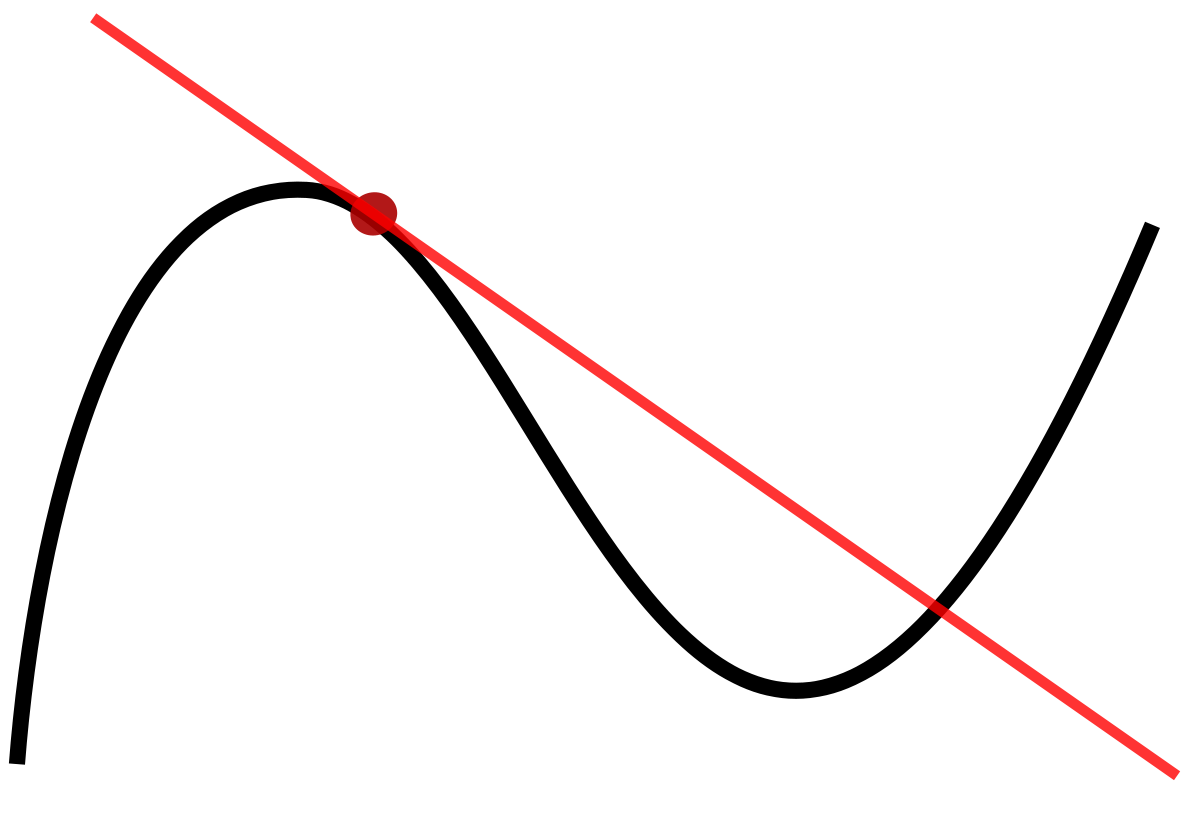
\includegraphics[width=0.4\linewidth]{tangent_to_curve}
			\caption{Curve and its tangent}
			\label{fig:tangenttocurve}
		\end{figure}
		
		Given a curve $\mathscr{L}$: $y = f(x)$ we can find a \emph{tangent} line $y = ax + b$ to the curve at point $x_0$. A tangent is such a line that touches the curve $\mathscr{L}$ at the point ($x_0$, $f(x)$) 
		
		\bigskip
		
		The tangent is such a line that touches the curve $\mathscr{L}$ at the point  ($x_0$, $f(x_0)$) and has the same \emph{rate of change} as the function at this point.
		
	\end{flushleft}
\end{frame}




\begin{frame}{Rate of change of a function}
	% \framesubtitle{Part 1}
	\begin{flushleft}
		
		What is a rate of change of a function? Consider function $y = f(x)$. How does $y$ changes if you increase $x$ a little?
		
		\bigskip
		
		We can ask about it in this way: Let  $\Delta y = f(x + \Delta x) - f(x)$, where $\Delta x$ is a small increase in $x$, and $\Delta y$ captures the corresponding increase in $y$. What is the ration of $\Delta y$ to $\Delta x$?
		
		\begin{equation}
			\frac{\Delta y}{\Delta x} = \frac{f(x + \Delta x) - f(x)}{\Delta x}
		\end{equation}
		
		
	\end{flushleft}
\end{frame}


\begin{frame}{Rate of change of a function}
	% \framesubtitle{Part 1}
	\begin{flushleft}
		
		\begin{figure}
			\centering
			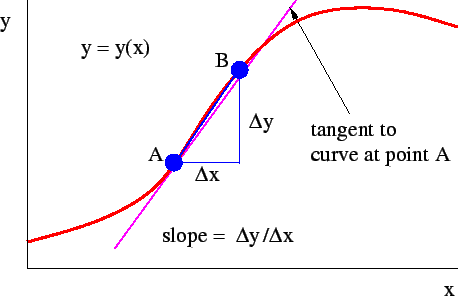
\includegraphics[width=0.65\linewidth]{tangent_to_curve2}
		\end{figure}
			
			Making $\Delta x$ smaller and smaller we find the true slope of the function: 
			
		\begin{equation}
			a = \lim_{\Delta x \to 0} \frac{f(x + \Delta x) - f(x)}{\Delta x}
		\end{equation}
		
	\end{flushleft}
\end{frame}

\begin{frame}{Rate of change of a function}
	% \framesubtitle{Part 1}
	\begin{flushleft}
		
		Notice that the tangent line to a function $y = f(x)$ at a point $x_0$ is given its equation:
		
		\begin{align}
			y = ax + b \\
			a =  \lim_{\Delta x \to 0} \frac{f(x_0 + \Delta x) - f(x_0)}{\Delta x} \\
			b = f(x_0) - a x_0
		\end{align} 
		
	\end{flushleft}
\end{frame}



\begin{frame}{Derivative}
	% \framesubtitle{Part 1}
	\begin{flushleft}
		
		We have a special name for this limit $\underset{\Delta x \to 0}{\lim} \frac{f(x + \Delta x) - f(x)}{\Delta x}$. We call it \emph{derivative of $f(x)$}.
		
		\bigskip
		
		\begin{block}{Derivative}
			$\frac{d}{dx} f(x) = \underset{\Delta x \to 0}{\lim} \frac{f(x + \Delta x) - f(x)}{\Delta x}$ is called a derivative of $f(x)$ with respect to $x$.
		\end{block}
		
		
		
	\end{flushleft}
\end{frame}



\begin{frame}{Derivative of a function, examples}
	% \framesubtitle{Part 1}
	\begin{flushleft}
		
		Consider a function $y = x$. What is its derivative?
		
		\begin{equation}
			\frac{d}{dx} x= \underset{\Delta x \to 0}{\lim} \frac{x + \Delta x - x}{\Delta x} = 1
		\end{equation}
	
	\bigskip
	
	Consider a function $y = 10 x$. What is its derivative?
	
	\begin{equation}
		\frac{d}{dx} 10x = \underset{\Delta x \to 0}{\lim} \frac{10 x + 10 \Delta x - 10 x}{\Delta x} = 10
	\end{equation}
		
	\end{flushleft}
\end{frame}




\begin{frame}{Derivative of a function, examples}
	% \framesubtitle{Part 1}
	\begin{flushleft}
		
		Consider a function $y = x^2$. What is its derivative?
		
		\begin{align*}
			\frac{d}{dx}  (x^2) = \underset{\Delta x \to 0}{\lim} \frac{(x + \Delta x)^2 - x^2}{\Delta x} = \\
			=\underset{\Delta x \to 0}{\lim} \frac{x^2 + 2 x  \Delta x+ \Delta x^2 - x^2}{\Delta x} = \\ 
			=\underset{\Delta x \to 0}{\lim} \frac{2 x  \Delta x}{\Delta x} + 
			\underset{\Delta x \to 0}{\lim} \frac{\Delta x^2}{\Delta x} = 2 x
		\end{align*}
		
		So, $\frac{d}{dx}  (x^2)  = 2x$.
		
	\end{flushleft}
\end{frame}








\begin{frame}{Properties of derivatives}
	% \framesubtitle{Part 1}
	\begin{flushleft}
		
		In general, derivatives have some interesting properties:
		
		\begin{block}{Distributive}
			$\frac{d}{dx} (f(x) + g(x)) = \frac{d}{dx} f(x) + \frac{d}{dx} g(x)$
		\end{block}
		\begin{block}{Multiplicative}
			$\frac{d}{dx} (a f(x) ) = a \frac{d}{dx} f(x) $
		\end{block}
	
		\bigskip
	
		In general, derivative is a linear operation.
		
	\end{flushleft}
\end{frame}



\begin{frame}{Derivatives of polynomials}
	% \framesubtitle{Part 1}
	\begin{flushleft}
		
		Consider a function $y = x^n$. Its derivative can be found as:
		
		\begin{block}{Derivative of $x^n$}
			$\frac{d}{dx}  x^n = n x^{n-1}$
		\end{block}
	
	\bigskip
		
		Let us see some examples:
		
		\begin{align}
			\frac{d}{dx}  x^7 = 7 x^6 \\
			\frac{d}{dx}  2 x^3 = 6 x^2 \\
			\frac{d}{dx}  (x^2 - x + 6) = 2x - 1
		\end{align}
		
		
	\end{flushleft}
\end{frame}


\begin{frame}{Derivatives and slopes}
	% \framesubtitle{Part 1}
	\begin{flushleft}
		
		Coming back to our original example. We want to find a tangent line to a function $y = f(x)$.
		
		\bigskip
		
		The slope of the tangent like is given by the derivative of  $y = f(x)$: $a = \frac{d}{dx} f(x)$, evaluated as the point $x_0$.
		
		\bigskip
		
		There are two equivalent ways to define the tangent line. First is to give it as $y = ax + b$, where $b = f(x_0) - a x_0$. Second is to give it as $y = a (x - x_0) + c$, where $c =  f(x_0)$. Both are used in practice.
		
	\end{flushleft}
\end{frame}


\begin{frame}{Derivatives and slopes}
	% \framesubtitle{Part 1}
	\begin{flushleft}
		
		Now we can find an angle between the slope of the tangent line and the horizon. How? Remember the second lecture: we find a vector on the line, in this case $[1, \ a]$ would do, and find an angle it makes with the horizontal vector $[1, \ 0]$ using dot product.
		
		\bigskip
		
		But we do not need to go by such a complicated rout. There is a property of a tangent line (which you can prove on your own) that the derivative of $y = f(x)$ is equal to the tangent of the angle between its slope and the horizon:
		
		\begin{equation}
			\tan (\varphi) = \frac{d}{dx} f(x)
		\end{equation}
		
	\end{flushleft}
\end{frame}


\begin{frame}{Derivatives and normals}
	% \framesubtitle{Part 1}
	\begin{flushleft}
		
		Knowing a tangent vector $[1, \ a]$ to a function $y = f(x)$ we can find a normal vector to that function. How? Remember that normal vector is orthogonal to a tangent vector, so we can find it by considering their dot product.
		
		\bigskip
		
		Why would you need to know normal vectors? In practice, they are needed for applications from 3D printing to walking robotics - in finding normals to surfaces. Consider a task: draw a curve that is one unit away from the curve $y = 10 x^2$ in the normal direction. See if you can solve it by using derivatives, tangents and normals.
		
		
	\end{flushleft}
\end{frame}



\begin{frame}{Thank you!}
\centerline{Lecture slides are available via Moodle.}
\bigskip
\centerline{You can help improve these slides at:}
\centerline{\mygit}
\bigskip
\centerline{Check Moodle for additional links, videos, textbook suggestions.}
\bigskip

\centerline{\textcolor{black}{\qrcode[height=1.6in]{https://github.com/SergeiSa/Extra-math-for-high-school}}}

\end{frame}

\end{document}
